%%
%% This is file `sample-sigconf.tex',
%% generated with the docstrip utility.
%%
%% The original source files were:
%%
%% samples.dtx  (with options: `sigconf')
%% 
%% IMPORTANT NOTICE:
%% 
%% For the copyright see the source file.
%% 
%% Any modified versions of this file must be renamed
%% with new filenames distinct from sample-sigconf.tex.
%% 
%% For distribution of the original source see the terms
%% for copying and modification in the file samples.dtx.
%% 
%% This generated file may be distributed as long as the
%% original source files, as listed above, are part of the
%% same distribution. (The sources need not necessarily be
%% in the same archive or directory.)
%%
%% The first command in your LaTeX source must be the \documentclass command.
\documentclass[manuscript]{acmart} %need to change [manuscript]
\newcommand{\squeezeup}{\vspace{-6mm}}
\newcommand{\squeezeuplittle}{\vspace{-3pt}}
\newcommand{\squeezeuphalf}{\vspace{-2mm}}
%% NOTE that a single column version is required for 
%% submission and peer review. This can be done by changing
%% the \doucmentclass[...]{acmart} in this template to 
%% \documentclass[manuscript,screen]{acmart}
%% 
%% To ensure 100% compatibility, please check the white list of
%% approved LaTeX packages to be used with the Master Article Template at
%% https://www.acm.org/publications/taps/whitelist-of-latex-packages 
%% before creating your document. The white list page provides 
%% information on how to submit additional LaTeX packages for 
%% review and adoption.
%% Fonts used in the template cannot be substituted; margin 
%% adjustments are not allowed.

%%
%% \BibTeX command to typeset BibTeX logo in the docs
\AtBeginDocument{%
  \providecommand\BibTeX{{%
    \normalfont B\kern-0.5em{\scshape i\kern-0.25em b}\kern-0.8em\TeX}}}

%% Rights management information.  This information is sent to you
%% when you complete the rights form.  These commands have SAMPLE
%% values in them; it is your responsibility as an author to replace
%% the commands and values with those provided to you when you
%% complete the rights form.
%%\setcopyright{acmcopyright}
%%\copyrightyear{2021}
%%\acmYear{2021}
%%\acmDOI{}

%% These commands are for a PROCEEDINGS abstract or paper.
%%\acmConference[SA '21]{SA ’21 Emerging Technologies}{December 14-17, 2021}{Tokyo, Japan}
%%\acmBooktitle{SA '21:  SIGGRAPH Asia 2021 Emerging Technologies (SA ’21 Emerging Technologies),
%%  December 14-17, 2021, Tokyo, Japan}
%%\acmPrice{15.00}
%%\acmISBN{}

\setcopyright{rightsretained}
\copyrightyear{2024}
\acmYear{2024}
\acmConference{(SIGGRAPH '24 Immersive Pavilion:}{July 28 - August 1, 2024}{Denver,
United States of America}
\acmBooktitle{SIGGRAPH 2024 Immersive Pavilion (SIGGRAPH '24 Immersive Pavilion),July 28 - August 1, 2024}
\acmDOI{10.1145/3476122.3484837}
\acmISBN{978-1-4503-8685-2/21/12}

%%
%% Submission ID.
%% Use this when submitting an article to a sponsored event. You'll
%% receive a unique submission ID from the organizers
%% of the event, and this ID should be used as the parameter to this command.
%%\acmSubmissionID{123-A56-BU3}

%%
%% The majority of ACM publications use numbered citations and
%% references.  The command \citestyle{authoryear} switches to the
%% "author year" style.
%%
%% If you are preparing content for an event
%% sponsored by ACM SIGGRAPH, you must use the "author year" style of
%% citations and references.
%% Uncommenting
%% the next command will enable that style.
\citestyle{acmauthoryear}

%%
%% end of the preamble, start of the body of the document source.
\begin{document}


%%
%% The "title" command has an optional parameter,
%% allowing the author to define a "short title" to be used in page headers.
\title{WaterForm: Altering the Liquid to Generate Multisensory Feedback for Enhancing Immersive Environment}

%Imports bibliography file
%%
%% The "author" command and its associated commands are used to define
%% the authors and their affiliations.
%% Of note is the shared affiliation of the first two authors, and the
%% "authornote" and "authornotemark" commands
%% used to denote shared contribution to the research.
\author{I-Chin Chen}
\affiliation{%
  \institution{National Taipei University of Technology}
  %\city{Taipei}
  \country{Taipei, Taiwan}
}

\author{Hsin-Chia Chang}
\affiliation{%
  \institution{National Taipei University of Technology}
  \country{Taipei, Taiwan}
  }

\author{Chia-Yi Hung}
\affiliation{%
  \institution{National Taipei University of Technology}
  \country{Taipei, Taiwan}
  }

\author{Chi-Yu Lin}
\affiliation{%
  \institution{National Taipei University of Technology}
  \country{Taipei, Taiwan}
  }
  
\author{Kuan-Ning Chang}
\affiliation{%
  \institution{National Taipei University of Technology}
  \country{Taipei, Taiwan}
  }

\author{Ping-Hsuan Han}
%\email{pinghsuan.han@gmail.com}
\affiliation{%
  \institution{National Taipei University of Technology}
  \country{Taipei, Taiwan}
  }
%%
%% By default, the full list of authors will be used in the page
%% headers. Often, this list is too long, and will overlap
%% other information printed in the page headers. This command allows
%% the author to define a more concise list
%% of authors' names for this purpose.
\renewcommand{\shortauthors}{I-Chin Chen, et al.}

%%
%% The abstract is a short summary of the work to be presented in the
%% article.
\begin{abstract}
With virtual reality head-mounted display and haptic technologies, we can create a compelling immersive experience. Thus, researchers have been exploring integrating different feedback modules to provide more abundantly hybrid feedback systems. On the other approach, they want to use the same module to generate multiple feedback with different interaction techniques. However, simultaneously providing multiple sensory feedbacks in virtual environments presents challenges beyond system integration and stability. Ensuring that users can experience multiple stimuli without compromising the overall immersive experience, as in a physical world, is still challenging. Therefore, we present WaterForm, a liquid-transformation system that utilizes the liquid to generate multisensory feedback, including water splash, water flow, gravity, wind, resistance, buoyant force, mechanical energy, and mist, to enhance the immersive environment. In our demonstration, we developed a VR excursion in the virtual East landscape for exploring self-awareness via immersive storytelling.
\vspace{-0.45em}
\end{abstract}



%%
%% The code below is generated by the tool at http://dl.acm.org/ccs.cfm.
%% Please copy and paste the code instead of the example below.
%%
\begin{CCSXML}
<ccs2012>
 <concept>
  <concept_id>10010520.10010553.10010562</concept_id>
  <concept_desc>Computer systems organization~Embedded systems</concept_desc>
  <concept_significance>500</concept_significance>
 </concept>
 <concept>
  <concept_id>10010520.10010575.10010755</concept_id>
  <concept_desc>Computer systems organization~Redundancy</concept_desc>
  <concept_significance>300</concept_significance>
 </concept>
 <concept>
  <concept_id>10010520.10010553.10010554</concept_id>
  <concept_desc>Computer systems organization~Robotics</concept_desc>
  <concept_significance>100</concept_significance>
 </concept>
 <concept>
  <concept_id>10003033.10003083.10003095</concept_id>
  <concept_desc>Networks~Network reliability</concept_desc>
  <concept_significance>100</concept_significance>
 </concept>
</ccs2012>
\end{CCSXML}

\ccsdesc[500]{Human-centered computing~Interaction paradigms}
\ccsdesc{Human-centered computing~Virtual Realty}
%%
%% Keywords. The author(s) should pick words that accurately describe
%% the work being presented. Separate the keywords with commas.
\keywords{Liquid-transformation Systems, Hybrid Feedback, Relaxation Application, Mixed Reality}

%% A "teaser" image appears between the author and affiliation
%% information and the body of the document, and typically spans the
%% page.
\begin{teaserfigure}
  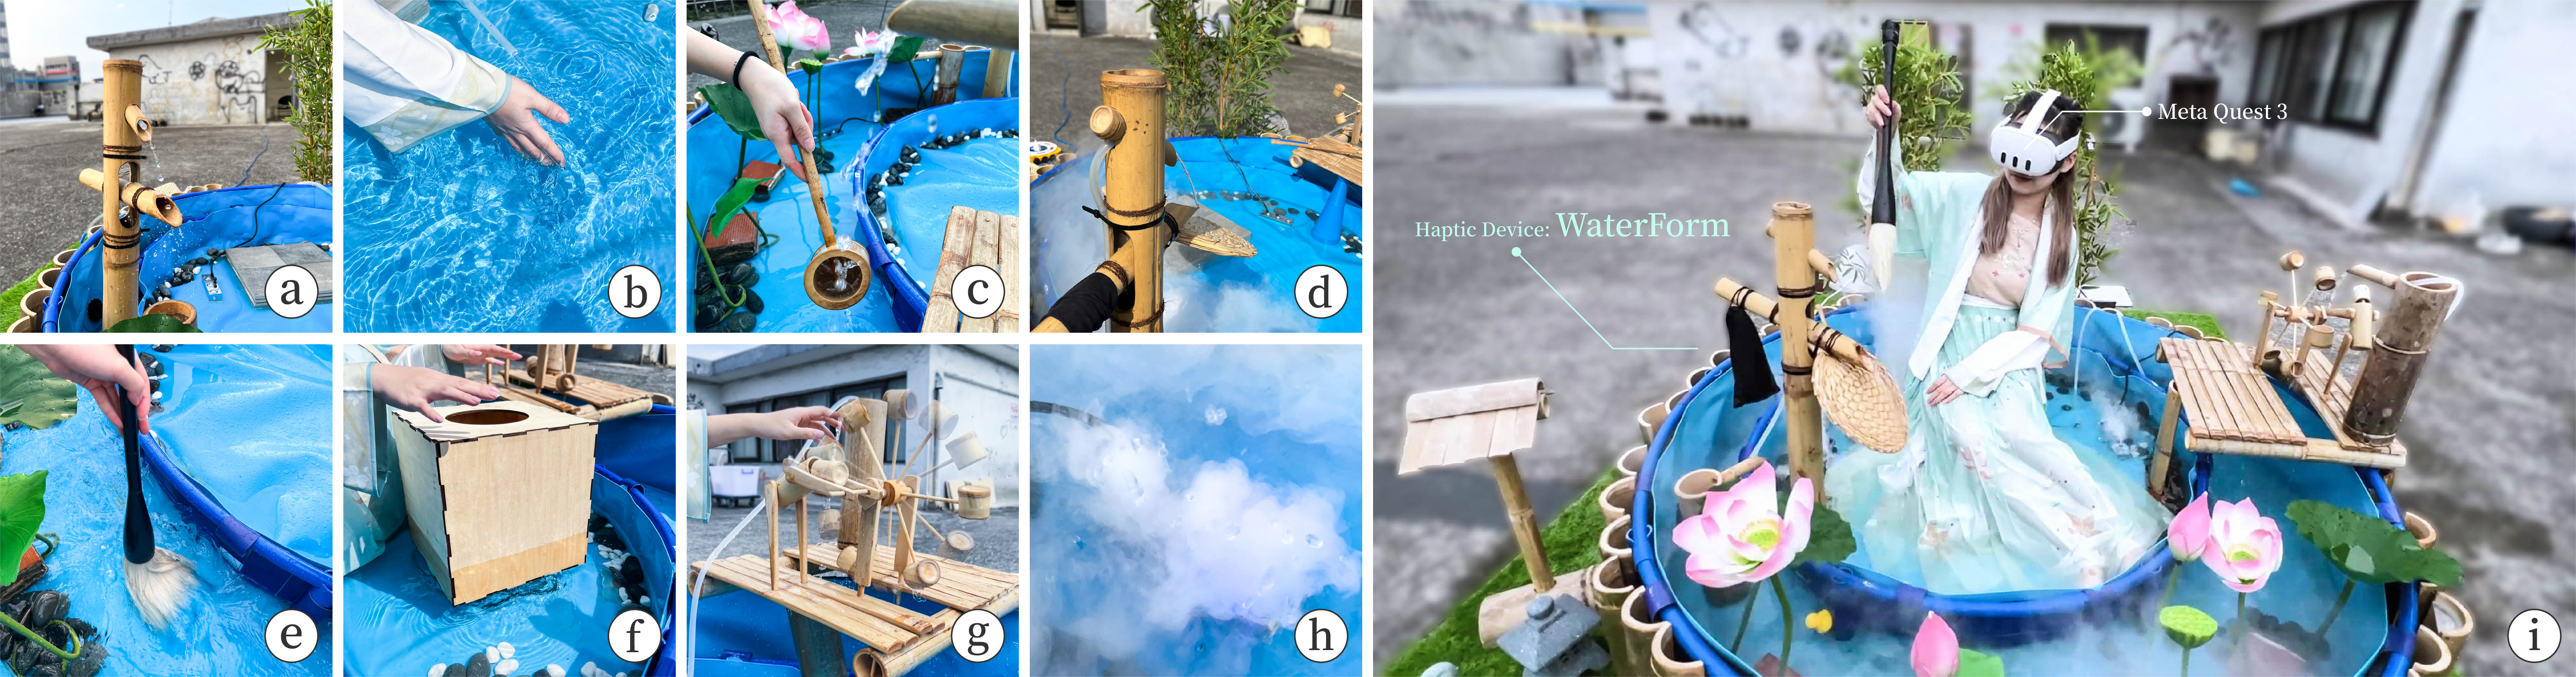
\includegraphics[width=\textwidth]{WF_SA.png}
  \vspace{-1.75em}
  \caption{Our Liquid-transformation Systems produces (a) water splash, (b) water flow, (c) gravity, (d) wind,  (e) resistance, (f) buoyant force, (g) mechanical energy, and (h) mist to enhance (i) immersive environment.}
  \vspace{0.5em}
  \Description{}
  \label{fig:teaser}
\end{teaserfigure}

%%
%% This command processes the author and affiliation and title
%% information and builds the first part of the formatted document.
\maketitle
\section{INTRODUCTION}
The research team has been devoted to providing various tactile experiences in virtual reality (VR) to enhance immersive experiences using different technologies. Additionally, liquid can directly or indirectly offer multisensory feedback through its charistic and transformation. GroundFlow \cite{han2023groundflow} proposes a liquid tactile floor system to simulate fluid on the ground in VR, employing multi-flow feedback mechanisms to allow users to explore rivers, beaches, and swimming pools. Lotus \cite{chen2018lotus} utilizes the transformation of liquid into mist, guided by airflow modules to simulate olfactory environments. AoEs \cite{han2017aoes} utilize tactile simulation integrated devices to create immersive environments, simultaneously providing cold and warm virtual environments. AquaTop Display \cite{matoba2013aquatop} uses water as the screen surface for projection systems, allowing users to interact immersively both above and below the water surface. 
%上面事都會接觸到水,這邊以下不會,所以這裡要寫一兩句說明。

In addition to techniques involving direct contact with water, previous research has also explored generating sensory feedback indirectly through the transformation of water. INVISIBLE \cite{nakano2006invisible} proposes a weight perception system where users experience weight through fluid transmission. GravityCup \cite{cheng2018gravitycup} and GravityPack \cite{chen2022gravitypack} introduce a portable gravity display that mimics grasping, holding, and releasing virtual objects in the virtual world using liquid simulation. Waving Blanket \cite{han2022waving} presents a dynamic fluid distribution system utilizing reconfigurable pipeline systems to explore mechanisms for simulating vibration, pressure, weight, and weight-shifting feedback. LiquidMask \cite{liao2019liquidmask} fills masks with liquid to generate thermal changes and vibrations.
%(V1 Contribution)
%However, researchers are still exploring the integration of different feedback modules to provide mixed feedback. One possible approach is to use the same module to generate multiple feedbacks, including water splash, water flow, gravity, wind, resistance, buoyant force, mechanical energy, and mist through different interaction techniques. Therefore, this paper designs and implements a liquid transformation system, WaterForm (\autoref{fig:teaser}i), utilizing water as a single module, to generate hybrid feedback by transforming liquid and enhancing immersive environments. Additionally, we develop a relaxation MR application to demonstrate the practicality of our device.

%(V2 Contribution)
While previous research cases have utilized various methods to transform water into different types of feedback, there has yet to be a system that provided by water simultaneously. One possible approach is to use the same module to generate multiple feedbacks simultaneously through different interaction techniques. Hence, this paper designs and implements a liquid transformation system, utilizing water as a single module, to generate water splashes, currents, gravity, wind, resistance, buoyancy, mechanical energy, mist, and more, enhancing immersive environments. Additionally, we develop a relaxation application to demonstrate the practicality of our device.

\vspace{-0.5em}
\section{DESIGN AND IMPLEMENTATION}
%\subsection{System Overview}
WaterForm is a liquid-based haptic system that utilizes the liquid to generate multisensory feedback, including water splash, water flow, gravity, wind, resistance, buoyant force, mechanical energy, and mist, to enhance the immersive environment (Fig 1.i). The device's overall dimensions are 3m * 3m * 0.8m, composed of internal and external water pools and modules. It primarily consists of an external water pool (1.57m * 1.57m * 0.35m) to store water and utilizes a high-power pump (BS6500, flow rate: 8.0L/min) to pump water to the internal water pool and various modules for transforming the liquid form. Users sit on diatomaceous earth (0.4m * 0.4m * 0.25m) stacked inside the internal water pool for the experience.

The maximum water level of the system is 0.15m, with two water pumps supplying water to the Jing-Lu and water wheel respectively. Water from the Jing-Lu falls from a height, creating water splash (Fig 1.a). Users can use water ladles to collect the water splashing down to experience gravity (Fig 1.c). By Applying weight behind the Jing-Lu and attacking a fan in front of the Jing-Lu, through the lever mechanism, the system can generate wind (Fig 1.d). The water-driven water wheel generates mechanical energy (Fig 1. g) by rotating the structure, and water drops create water flow (Fig 1.b) as they fall. The Atomizers (M-1007) placed 0.02m underwater generate mist  (Fig 1.h). By pumping water from the external pool to the internal pool, users can experience a buoyant force (Fig 1.f). Furthermore, users can use a writing brush in the water to feel resistance (Fig 1.e). Our device achieves liquid transformation simulation through the Unity and Linkit 7697 Bluetooth software operating system.

%\subsection{landscaping design (Decoration)}
In addition, elements of Chinese Taoist philosophy are incorporated into the landscape design of the pond. Surrounding the pond are embellishments such as lotus, bamboo, and stone lanterns, creating an overall serene atmosphere. Within the pond, the inner portion features landscapes of mountains and dry elements, representing the white portion of the Tai Chi diagram, symbolizing "yang"; while the outer portion is represented by water, symbolizing the black portion, "yin." The interaction and flow between the inner and outer ponds serve as a medium for harmonizing the yin and yang, allowing users to experience moments of balance and, at times, new and different sensations amidst conflicts and contradictions, thus exploring the inner self.

\section{APPLICATION: Relaxation Application}
To demonstrate our concept, we design a VR excursion in the virtual East landscape with multisensory feedback. Users will wear the HMD (Meta Quest 3) while seated within our device. Based on our WaterForm system, we create two virtual environments (VE) and eight interactive modes with mixed reality (MR). In these VE, users can immerse themselves in serene surroundings, such as sitting by a pavilion enjoying the tranquil scenery and freely interacting with physical devices from the real world. Guided prompts will direct users to focus on sensory changes in the present moment, facilitating exploration between the virtual and physical realms.

\section{DISCUSSION AND FUTURE WORK}
This work proposes a Liquid-transformation Systems to enhance immersive experiences with hybrid tactile sensation feedback, including water splash, water flow, gravity, wind, resistance, buoyant force, mechanical energy, and mist. By wearing the HMD, users can sit within our device to perceive different haptic experiences in our relaxation application. In the future, we will conduct user studies to understand how different senses affect the perceived level of relaxation, and apply these findings to applications such as flow state, mindfulness, meditation, and more.

%%
%% The next two lines define the bibliography style to be used, and
%% the bibliography file.
\bibliographystyle{ACM-Reference-Format}
\bibliography{sample-base}

%%
%% If your work has an appendix, this is the place to put it.
\appendix

\end{document}
\endinput
%%
%% End of file `sample-sigconf.tex'.